% main.tex
% Standalone demonstration file for the CERI-modified University of Memphis
% dissertation/thesis LaTeX template.
%
% Compiled and developed by Navin Thapa.
% Updated against the public University of Memphis Graduate School
% Thesis/Dissertation Preparation Guide, last revised October 2025.
%
% This is NOT an official University of Memphis, Graduate School, or CERI
% template. Use at your own risk. Always confirm final requirements with the
% Graduate School and your advisor/committee.
%
% Overleaf settings:
%   Compiler: LuaLaTeX
%   TeX Live: 2025 or Rolling
%   Main document: main.tex
%   Bibliography: BibTeX
%
% Accessibility/PDF tagging metadata must appear before \documentclass.
% On the newest Overleaf/Rolling TeX Live, you may replace the testphase line
% with: tagging=on
\DocumentMetadata{
  lang=en-US,
  pdfstandard=ua-2,
  pdfversion=2.0,
  testphase={phase-III,math,table,title,firstaid}
}

% Options:
%   doctoral/master       dissertation or thesis wording
%   fulldocument/proposal final document or proposal wording
%   secnum/nosecnum       numbered or unnumbered section headings
%   pdfonly/boundcopy     1-inch left margin or 1.5-inch bound-copy margin
%   boundcover/noboundcover legacy title-page horizontal offset option
\documentclass[doctoral,fulldocument,secnum,pdfonly,boundcover]{uofm}

% -----------------------------------------------------------------------------
% Dissertation metadata for the title page
% -----------------------------------------------------------------------------
\title{A Sample Dissertation Title Written in Title Case}
\author{Student Name}
\degree{Doctor of Philosophy}
\major{Program Name}
\advisor{Advisor Name}
\date{Month Year}

% -----------------------------------------------------------------------------
% Packages for examples only. The class already loads the core formatting
% packages needed for the UofM/CERI legacy format.
% -----------------------------------------------------------------------------
\usepackage{siunitx}
\sisetup{detect-all=true}

% Citation punctuation: AGU-like author-year style using natbib and uomagu.bst.
\bibpunct{(}{)}{;}{a}{,}{,}

\begin{document}

% =============================================================================
% TITLE AND PRELIMINARY PAGES
% =============================================================================

% Title page is counted as Roman i, but the page number is hidden.
\maketitle

% Preliminary pages begin with Roman page ii.
\frontmatter

% Optional copyright page. Delete/comment out if not needed.
\copyrightpage

% Optional dedication page. Delete/comment out if not needed.
\begin{dedication}
Lorem ipsum dolor sit amet, consectetur adipiscing elit. Integer non sem vitae
ligula tempor consequat. Donec vitae augue sit amet lorem facilisis pulvinar.
\end{dedication}

% Optional acknowledgments page.
\begin{acknowledgments}
Lorem ipsum dolor sit amet, consectetur adipiscing elit. Phasellus tincidunt,
metus vitae consequat volutpat, velit arcu tincidunt lectus, at laoreet magna
nisl sed justo. Vestibulum ante ipsum primis in faucibus orci luctus et ultrices
posuere cubilia curae; Integer vitae magna at est tincidunt sodales. Curabitur
id mi vitae lorem ullamcorper luctus.
\end{acknowledgments}

% Required if journal articles are used as dissertation/thesis chapters.
\begin{preface}
Lorem ipsum dolor sit amet, consectetur adipiscing elit. This sample preface
shows where the author may describe the scope and purpose of the manuscript.
If journal articles are used as chapters, replace this paragraph with the names
of the journals, the publication or submission status of each manuscript chapter,
and any information requested by the Graduate School or committee.
\end{preface}

% Abstract: maximum 350 words. Do not include headings, citations, equations,
% formulas, figures, diagrams, or tables inside the abstract.
\begin{abstract}
Lorem ipsum dolor sit amet, consectetur adipiscing elit. Sed vitae magna nec
ipsum ultricies fermentum. Praesent tempor, mi vitae aliquam volutpat, lectus
urna convallis lorem, ac bibendum nulla erat vitae velit. Integer consequat
sapien sed neque faucibus, non imperdiet arcu feugiat. Donec facilisis, sapien
non vulputate posuere, erat lectus pellentesque magna, sed dictum lacus mi vitae
nibh. Nulla facilisi. Cras sed luctus est. Proin luctus, massa sed vestibulum
venenatis, nisl augue viverra arcu, eget porta risus est sed nibh. Aenean
volutpat ex sed turpis suscipit, vitae gravida neque pretium. Maecenas sed dui
vitae velit luctus dictum. Suspendisse potenti. Etiam ac augue at erat pulvinar
convallis. This abstract is placeholder text only and should be replaced with a
clear summary of the purpose, approach, major findings, and conclusions of the
final work.

% Optional keywords example. Delete if your program does not want keywords.
\begin{keywords}
keyword one; keyword two; keyword three; keyword four
\end{keywords}
\end{abstract}

% Required generated lists. Remove List of Tables/List of Figures only if your
% final document has fewer than five tables/figures and your department permits
% omission.
\tableofcontents
\listoftables
\listoffigures

% Optional list of abbreviations. Delete/comment out if not needed.
\begin{abbreviations}
\begin{tabular}{@{}ll@{}}
ADA & Americans with Disabilities Act\\
CERI & Center for Earthquake Research and Information\\
ETD & Electronic Thesis or Dissertation\\
PDF & Portable Document Format\\
UofM & University of Memphis
\end{tabular}
\end{abbreviations}

% =============================================================================
% MAIN TEXT
% =============================================================================

% Main text begins with Arabic page 1.
\mainmatter

\chapter{Introduction}

Lorem ipsum dolor sit amet, consectetur adipiscing elit. Curabitur at augue vel
nisl tempor vulputate. Donec vel mi eget sem blandit fermentum. This sentence
shows an author--year citation using the bundled bibliography style
\citep{uomGuide2025}. Another sentence demonstrates a citation to current
LaTeX accessibility work \citep{latexTaggingProject}.

\section{Background and Motivation}

Lorem ipsum dolor sit amet, consectetur adipiscing elit. Pellentesque habitant
morbi tristique senectus et netus et malesuada fames ac turpis egestas. Sed
consequat urna quis augue volutpat, a ultricies sapien consectetur. This
sentence includes a sample footnote for checking footnote spacing and numbering.\footnote{Lorem ipsum dolor sit amet, consectetur adipiscing elit.}

\subsection{Example Subsection}

Lorem ipsum dolor sit amet, consectetur adipiscing elit. Integer non urna sed
ligula facilisis pulvinar. If the Graduate School or committee asks for no
numbered subheadings, change the class option from \texttt{secnum} to
\texttt{nosecnum}.

\section{Example Quotation}

The following quotation environment demonstrates block quotation formatting.
Replace it with quoted material only when the final dissertation requires it and
when proper citation and permissions have been checked.

\begin{quote}
Lorem ipsum dolor sit amet, consectetur adipiscing elit. Suspendisse potenti.
Praesent mattis urna sed sem facilisis, vitae elementum nibh posuere.
\end{quote}

\chapter{Example Manuscript-Style Chapter}

\section*{Author Contribution Statement}
Lorem ipsum dolor sit amet, consectetur adipiscing elit. Replace this sample
statement with the exact author contribution statement required for a coauthored
manuscript-style chapter. Include the student's role and the roles of coauthors
as approved by the advisor and committee.

\section{Example Figure with Alt Text}

Lorem ipsum dolor sit amet, consectetur adipiscing elit. Figure~\ref{fig:sample}
shows how to insert a standard LaTeX figure with alternative text. The visible
caption remains below the figure, and the accessibility description is placed in
the \texttt{alt=\{...\}} option of \texttt{\textbackslash includegraphics}.

\begin{figure}[htbp]
\centering
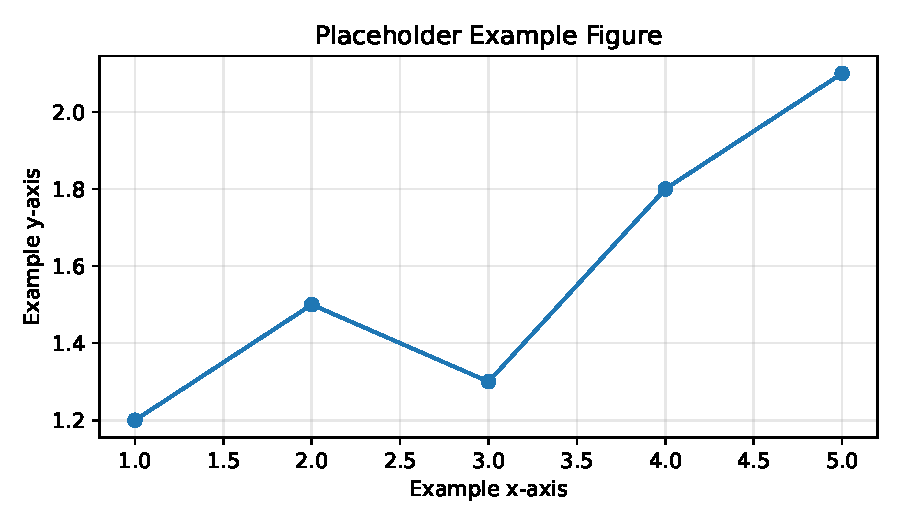
\includegraphics[
  width=0.82\textwidth,
  alt={Placeholder line plot with five circular markers connected by a line. The example demonstrates where a scientific figure description should be written for screen-reader users.}
]{figures/example_figure.pdf}
\caption{Example figure caption. Replace this placeholder figure and caption with the final dissertation figure and caption.}
\label{fig:sample}
\end{figure}

\section{Example Accessible Table}

Lorem ipsum dolor sit amet, consectetur adipiscing elit. Table~\ref{tab:sample}
shows a simple data table. For tagged PDF output, the line immediately before
the \texttt{tabular} environment identifies the first row as the header row.

\begin{table}[htbp]
\caption{Example table caption. Replace this placeholder with the final dissertation table caption.}
\label{tab:sample}
\centering
\tagpdfsetup{table/header-rows={1},table/header-columns={1}}
\begin{tabular}{@{}lccc@{}}
\toprule
Sample & Value A & Value B & Category \\
\midrule
Item 1 & 10 & 0.25 & Alpha \\
Item 2 & 15 & 0.40 & Beta \\
Item 3 & 20 & 0.55 & Gamma \\
Item 4 & 25 & 0.70 & Delta \\
\bottomrule
\end{tabular}
\end{table}

\section{Example Equation}

Lorem ipsum dolor sit amet, consectetur adipiscing elit. Equation~\ref{eq:sample}
shows a centered equation with a right-aligned number.

\begin{equation}
Y = aX + b
\label{eq:sample}
\end{equation}

Lorem ipsum dolor sit amet, consectetur adipiscing elit. Vestibulum nec arcu nec
nisi vestibulum pharetra. Mauris sed justo ac neque gravida tincidunt.

\chapter{Example Results Chapter}

\section{Example Results Text}

Lorem ipsum dolor sit amet, consectetur adipiscing elit. Sed sodales faucibus
orci, non facilisis velit eleifend a. Suspendisse nec orci lacus. Aliquam erat
volutpat. Donec in metus sed nibh volutpat lacinia.

\section{Example Visually Numbered Conclusions}

The following visually numbered paragraphs avoid list-tag warnings in some PDF
accessibility checkers while preserving a numbered appearance.

\noindent\textbf{1.} Lorem ipsum dolor sit amet, consectetur adipiscing elit.

\noindent\textbf{2.} Integer euismod augue vitae nibh convallis, nec fermentum
mauris dignissim.

\noindent\textbf{3.} Morbi suscipit orci at tellus volutpat, in pulvinar libero
consequat.

\chapter{Overall Discussion and Conclusions}

Lorem ipsum dolor sit amet, consectetur adipiscing elit. Praesent ac ligula et
massa pellentesque efficitur. Aliquam tempor, mi non cursus iaculis, urna nibh
condimentum purus, ac porta ligula sapien id nibh.

Lorem ipsum dolor sit amet, consectetur adipiscing elit. Donec et metus at lorem
volutpat vehicula. Sed in ultrices turpis. Vivamus sed pulvinar arcu. This
chapter demonstrates the required overall synthesis/conclusion chapter for a
manuscript-style dissertation.

% =============================================================================
% REFERENCES
% =============================================================================

\bibliographystyle{uomagu}
\bibliography{references}

% =============================================================================
% APPENDICES
% =============================================================================

\appendix

\chapter{Example Appendix}

Lorem ipsum dolor sit amet, consectetur adipiscing elit. Appendices may include
supplementary methods, extended tables, derivations, calibration information, or
additional figures that support the main document.

\section{Example Appendix Section}

Lorem ipsum dolor sit amet, consectetur adipiscing elit. Integer non sapien
rutrum, pretium mi non, porttitor ligula. Donec maximus leo in tortor porta,
nec pretium magna porta.

\end{document}
